\documentclass[11pt,paper=letterpaper,answers]{exam}
\usepackage{graphicx,lastpage}
\usepackage{upgreek}
\usepackage{censor}
\usepackage{amsmath}
\usepackage{mathtools}
\usepackage[spanish,es-tabla]{babel}
\usepackage{pdfpages}
\usepackage{tabularx}
\usepackage{graphicx}
\usepackage{adjustbox}
\usepackage{xcolor}
\usepackage{colortbl}
\usepackage{rotating}
\usepackage{multirow}
\usepackage[utf8]{inputenc}
\usepackage{moreverb}
\usepackage{enumitem}
\usepackage{float}

\renewcommand{\tablename}{Tabla}

\censorruledepth=-.2ex
\censorruleheight=.1ex
\hyphenpenalty 10000
\usepackage[paperheight=27.94cm,paperwidth=21.59cm,bindingoffset=0in,left=2.5cm,right=2.0cm, top=2cm,bottom=2cm, headsep=.5\baselineskip]{geometry}
\flushbottom
\usepackage[normalem]{ulem}
\renewcommand\ULthickness{2pt} 
\setlength\ULdepth{1.5ex}
\renewcommand{\baselinestretch}{1}
\pagestyle{empty}
\pagestyle{headandfoot}
\headrule
\newcommand{\continuedmessage}{%
\ifcontinuation{\footnotesize CGB }{}%
 }
\runningheader{\footnotesize Redes de Datos}
{\footnotesize Sem. X--- Laboratorio nro. X}
{\footnotesize P\'agina \thepage\ de \numpages}
\footrule
\footer{\footnotesize }
{}
{\ifincomplete{\footnotesize CG}{\iflastpage{\footnotesize Fin de Laboratorio nro X}{\footnotesize }}}
\usepackage{cleveref}
\crefname{figure}{figure}{figures}
\crefname{question}{question}{questions}

%==============================================================

\begin{document}

\noindent
\begin{minipage}[l]{.1\textwidth}%
\noindent
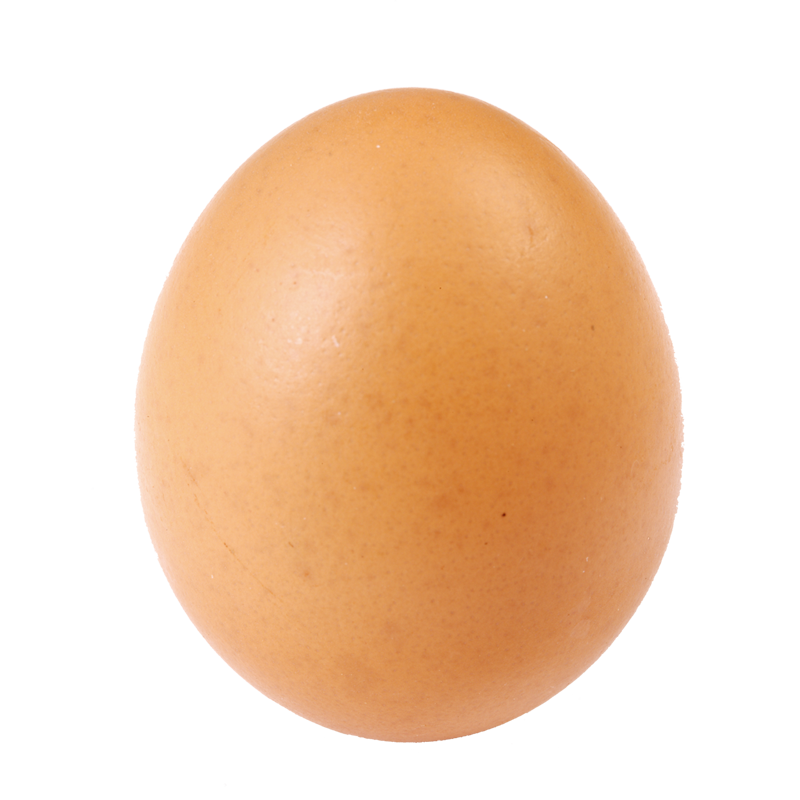
\includegraphics[scale = 0.1]{huevo.png} //aqui colocar el logo correspondiente
\end{minipage}
\hfill
\begin{minipage}[l]{0.9\textwidth}%
\begin{center}
{\Large \bfseries Escuela de Ingenier\'ia en Inform\'atica y Telecomunicaciones \par
\Large Universidad Free Code \\[2pt]
\large Redes de Datos {(\small Code: CIT-2114)}  \par
\vspace{0.2cm}
\Large Laboratorio X: INDICAR LABORATORIO” \par}
\vspace{0.0cm}
\end{center}
\end{minipage}

%\small {Nombre: \underline{\hspace{5cm}}} \hfill \footnotesize {RUT:\underline{\hspace{5cm}}
\vspace{0.5cm}
\par
\noindent
\uline{\normalsize {INDICAR FECHA} \hfill \footnotesize {} \hfill \footnotesize {}}

\vspace{0.5cm}

\pointsinrightmargin
\pointsdroppedatright
\marksnotpoints
\marginpointname{ puntos}
\pointpoints{mark}{marks}
\pointformat{\boldmath\themarginpoints}
\bracketedpoints

\renewcommand{\choicelabel}{\thechoice)}

\textbf{Grupo 1 - Sección 1. Integrantes: Prototipo}


\textbf{Emails: prototipo@mail.udp.cl}
\section{Objetivos y alcances}

\begin{itemize}
\item Obj1  
\item Obj2  
\item Obj3
\item Obj4
\item Ob5
\end{itemize}

\section{Introducción y Equipos}

Introduccion y equipos de los participantes



Computador 1:

CPU: AMD Ryzen 3 3300x

Ram: 16GB

OS: Windows 10\\



Computador 2:

CPU: Intel(R) Core(TM) i7-7500U

Ram: 8GB

OS: Windows 10\\



Computador 3:

CPU: AMD Ryzen 5 5600x

Ram: 32GB 

OS: Windows 10\\




\section{Materia - Indicar materia}
\subsection{
//colocar la wea aqui
}
}

\section{Conclusiones y comentarios}{

Indicar conclusiones y comentarios


}

\end{document} 